\section{Ziel}
\label{sec:Ziel}
In diesem Versuch werden die gleichsinnige-, die gegensinnige- und die gekoppelte Schwingung zweier Fadenpendel, die über eine Feder gekoppelt sind, untersucht. 
Ziel ist es die Schwingungs- bzw. Schwebungsdauer der genannten Schwingungsarten zu bestimmen. Daraus können Rückschlüsse über die Kopplungskonstante der Feder getroffen werden
und die Messwerte mit den Theoriewerten verglichen werden.

\section{Theorie}
\label{sec:Theorie}
Ein einzelnes Fadenpendel im Schwerefeld der Erde habe die Masse $m$, eine Fadenlänge $l$ und sei reibungsfrei aufgehängt. Bei einer Auslenkung um einen kleinen Winkel aus der 
Ruhelage wirkt ein Drehmoment $M = D_{\text{p}} \cdot \phi$, welches aus der Gewichtskraft resultiert, auf die Masse. $D_{\text{p}}$ ist die Winkelrichtgröße des Pendels und $\phi$
beschreibt den Auslenkwinkel. Mit der Kleinwinkelnäherung $\sin(x) \approx x$ folgt die Differentialgleichung eines harmonischen Oszillators für den Winkel $\phi$. Sie wird
gelöst durch eine harmonische Schwingung mit der Kreisfrequenz
\begin{equation}
    \label{eqn:omega}
    \omega = \sqrt{\frac{g}{l}} \qquad \text{und der Schwingungsdauer} \qquad T = \frac{1}{f} = \frac{2\pi}{\omega} = 2\pi \sqrt{\frac{l}{g}} .
\end{equation} 
Bei der Kopplung zweier identischer Fadenpendel mit einer Feder wirkt zusätzlich ein Drehmoment $M_1 = D_{\text{F}} (\phi_2 - \phi_1)$ bzw. $M_2 = - M_1$ auf die Pendel 1 und 2. 
Damit ergibt sich ein System gekoppelter Differentialgleichungen
\begin{align*}
    J \ddot\phi_1 + D_{\text{p}} \phi_1 &= D_{\text{F}}(\phi_2 - \phi_1) \\
    J \ddot\phi_2 + D_{\text{p}} \phi_2 &= D_{\text{F}}(\phi_1 - \phi_2)
\end{align*}
für die Auslenkwinkel $\phi_1$ und $\phi_2$ der beiden Pendel.$J$ ist das Trägheitsmoment der Pendel. Die Lösungen dieses Systems lassen sich als Überlagerung von Eigenschwingungen der beiden
Pendel darstellen. Es ergibt sich für jedes Pendel eine harmonische Schwingung mit den Frequenzen $\omega_1$ und $\omega_2$. Wenn $\alpha_1$ und $\alpha_2$ die Auslenkwinkel der
Pendel beschreiben, ist durch die Anfangsbedigungen $\alpha(t = 0)$ und $\dot\alpha(t = 0)$ eine eindeutige Lösung bestimmt. Unter diesen Lösungen werden verschiedene Schwingungsarten
mit speziellen Anfangsbedigungen unterschieden, die im folgenden diskutiert werden.

\begin{itemize}
    \item \textbf{Gleichsinnige Schwingung:} $\alpha_1 = \alpha_2$ \\
    Bei der gleichsinnigen Schwingung (\autoref{fig:Gleichsinnig}) werden beide Pendel um den Winkel $\alpha_1 = \alpha_2$ ausgelenkt. Die Pendel schwingen nun im gleichen Takt und beeinflussen sich nicht.
    Es wird also keine Kraft über die Feder übertragen. Die Schwingungsfrequenz entspricht der eines einzelnen Pendels (vgl. \autoref{eqn:omega}) und wird mit $\omega_+$ bezeichnet.

    \item \textbf{Gegensinnige Schwingung:} $\alpha_1 = -\alpha_2$ \\
    Bei dieser Schwingungsvariante (\autoref{fig:Gegensinnig}) werden die Pendel um den gleichen Winkel in entgegengesetzte Richtungen ausgelenkt. Über die Feder wirken nun betragsmäßig gleiche,
    entgegengerichtete Kräfte auf die Pendel. Dies hat zur Folge, dass die Pendel symmetrisch zu der Achse zwischen den Pendeln schwingen. Die Schwingungsfrequenz 
    \begin{gather}
        \label{eqn:omega_Gegensinnig}
        \omega_- = \sqrt{\frac{g + 2K}{l}}
    \end{gather}
    und die daraus resultierende Schwingungsdauer $T_-$ sind nun abhängig von der Federkonstante $K$. 
    
    \item \textbf{Gekoppelte Schwingung:} $\alpha_1 = 0, \, \alpha_2 \neq 0$ \\
    Für die gekoppelte Schwingung --auch Schwebefall genannt-- (\autoref{fig:Schwebung}) wird nur ein Pendel aus der Ruhelage ausgelenkt. Das Ausgelenkte Pendel fängt an zu schwingen und überträgt seine 
    kinetische Energie über die Kopplungsfeder an das zuerst ruhende Pendel. Dadurch wird die Schwingungsamplitude des ausgelenkten Pendels kontinuierlich kleiner, während
    die des zuerst Ruhenden zunimmt. Hat das ausgelenkte Pendel seine Energie vollständig abgegeben, blebt es stehen und die Amplitude des zweiten Pendels erreicht ihr Maximum.
    Anschließend beginnt der Prozess mit nun getauschten Ausgangspositionen von vorne. Dieses Phänomen wird als Schwebung bezeichnet. Die Schwebungsdauer $T_{\text{S}}$ bezeichnet 
    die Dauer einer Periode dieses Prozesses, also die Zeit von Ruhelage bis ernueter Ruhelage eines Pendels. Die Schwebungsfrequenz
    \begin{gather}
        \label{eqn:Schwebung}
        \omega_{\text{S}} = \omega_- - \omega_+ \qquad \text{und die Dauer} \qquad T_{\text{S}}  = \frac{T_+ \cdot T_-}{T_+ - T_-}
    \end{gather}
    lassen sich durch die Schwingungsdauern $T_+$ und $T_-$ der beiden anderen Fälle bestimmen.
    Aus den genannten Frequenzen kann ebenfalls die Federkonstante
    \begin{equation}
        \label{eqn:Federkonstante}
        K = \frac{\omega_-^2 - \omega_+^2}{\omega_-^2 + \omega_+^2} = \frac{T_+^2 - T_-^2}{T_+^2 + T_-^2}
    \end{equation}
    bestimmt werden.
\end{itemize}

\begin{figure}
    \centering
    \begin{subfigure}{.3\textwidth}
      \centering
      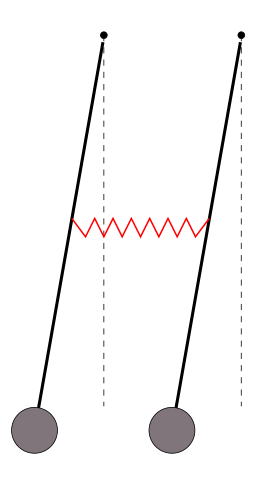
\includegraphics[width=.3\linewidth]{content/GleichsinnigeSchwingung.png}
      \caption{Gleichsinnig}
      \label{fig:Gleichsinnig}
    \end{subfigure}%
    \begin{subfigure}{.3\textwidth}
      \centering
      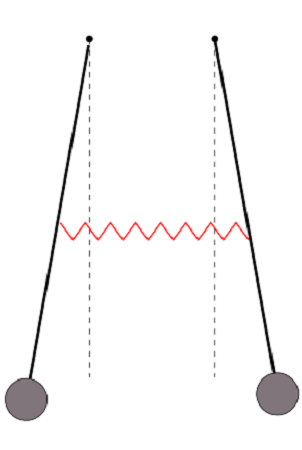
\includegraphics[width=.3\linewidth]{content/GegensinnigeSchwingung.png}
      \caption{Gegensinnig}
      \label{fig:Gegensinnig}
    \end{subfigure}
    \begin{subfigure}{.3\textwidth}
        \centering
        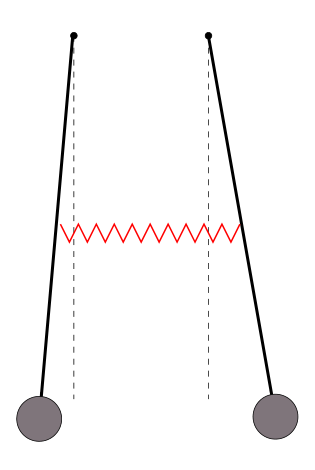
\includegraphics[width=.3\linewidth]{content/GekoppelteSchwingung.png}
        \caption{Gekoppelt / Schwebung}
        \label{fig:Schwebung}
      \end{subfigure}
    \caption{Die Schwingungsarten des Doppelpendels. \cite{v106}}
    \label{fig:Schwingungen}
\end{figure}